\documentclass[a4paper,11pt,fleqn,dvipsnames,twoside, openright ]{memoir} 	% Openright aabner kapitler paa hoejresider (openany begge)

%%%% PACKAGES %%%%

% ¤¤ Oversaettelse og tegnsaetning ¤¤ %
\usepackage[utf8]{inputenc}					% Input-indkodning af tegnsaet (UTF8)
\usepackage[english]{babel}					% Dokumentets sprog
\usepackage[T1]{fontenc}					% Output-indkodning af tegnsaet (T1)
\usepackage{ragged2e,anyfontsize}			% Justering af elementer
\usepackage{fixltx2e}						% Retter forskellige fejl i LaTeX-kernen
\usepackage{lscape}                         % For portræt mode i sideopsætning

% ¤¤ Figurer, tabeller (floats) og listings ¤¤ %
\usepackage{graphicx} 						% Haandtering af eksterne billeder (JPG, PNG, EPS, PDF)
\usepackage{epstopdf}
%\usepackage{eso-pic}						% Tilfoej billedekommandoer paa hver side
%\usepackage{wrapfig}						% Indsaettelse af figurer omsvoebt af tekst. \begin{wrapfigure}{Placering}{Stoerrelse}
\usepackage{multirow}                		% Fletning af raekker og kolonner (\multicolumn og \multirow)
\usepackage{multicol}         	        	% Muliggoer output i spalter
\usepackage{rotating}						% Rotation af tekst med \begin{sideways}...\end{sideways}
\usepackage{colortbl} 						% Farver i tabeller (fx \columncolor og \rowcolor)
\usepackage[table]{xcolor}					% Definer farver med \definecolor. Se mere: http://en.wikibooks.org/wiki/LaTeX/Colors
\definecolor{lightgray}{gray}{0.9}
\usepackage{flafter}						% Soerger for at floats ikke optraeder i teksten foer deres reference
\let\newfloat\relax 						% Justering mellem float-pakken og memoir
\usepackage{float}							% Muliggoer eksakt placering af floats, f.eks. \begin{figure}[H]
\usepackage{placeins}                       % \FloatBarrier
\usepackage{bytefield}                      %% Use for drwawing network packages
\usepackage{gensymb}
\usepackage{etex}                           % Er med for at få bytefields til at virke med hele gruppens LaTeX installationer.
\usepackage{listings}						% Placer kildekode i dokumentet med \begin{lstlisting}...\end{lstlisting}


% ¤¤ Matematik mm. ¤¤
\usepackage{amsmath,amssymb,stmaryrd} 		% Avancerede matematik-udvidelser
\usepackage{mathtools}						% Andre matematik- og tegnudvidelser
\usepackage{textcomp}                 		% Symbol-udvidelser (f.eks. promille-tegn med \textperthousand )
\usepackage{rsphrase}						% Kemi-pakke til RS-saetninger, f.eks. \rsphrase{R1}
\usepackage[version=3]{mhchem} 				% Kemi-pakke til flot og let notation af formler, f.eks. \ce{Fe2O3}
\usepackage{siunitx}						% Flot og konsistent praesentation af tal og enheder med \si{enhed} og \SI{tal}{enhed}
\sisetup{output-decimal-marker = {,}}		% Opsaetning af \SI (DE for komma som decimalseparator)

% ¤¤ Referencer og kilder ¤¤ %
\usepackage[english]{varioref}				% Muliggoer bl.a. krydshenvisninger med sidetal (\vref)
%\usepackage{natbib}							% Udvidelse med naturvidenskabelige citationsmodeller
\usepackage[style=numeric,natbib=true,backend=bibtex,bibencoding=ascii,sorting=none,maxnames=99,maxcitenames=1]{biblatex}
\usepackage{csquotes}
%\usepackage{xr}							% Referencer til eksternt dokument med \externaldocument{<NAVN>}

% ¤¤ Misc. ¤¤ %
\usepackage{lipsum}							% Dummy text \lipsum[..]
\usepackage[shortlabels]{enumitem}			% Muliggoer enkelt konfiguration af lister
\usepackage{pdfpages}						% Goer det muligt at inkludere pdf-dokumenter med kommandoen \includepdf[pages={x-y}]{fil.pdf}
\pdfoptionpdfminorversion=6					% Muliggoer inkludering af pdf dokumenter, af version 1.6 og hoejere
\pretolerance=2500 							% Justering af afstand mellem ord (hoejt tal, mindre orddeling og mere luft mellem ord)

% Kommentarer og rettelser med \fxnote. Med 'final' i stedet for 'draft' udloeser hver note en error i den faerdige rapport.
\usepackage[footnote,draft,english,silent,nomargin]{fixme}
%%%% CUSTOM SETTINGS %%%%

%%%% New Commands %%%%
\newcommand{\name}{\#NAME\#}

% ¤¤ Marginer ¤¤ %
\setlrmarginsandblock{3.5cm}{2.5cm}{*}		% \setlrmarginsandblock{Indbinding}{Kant}{Ratio}
\setulmarginsandblock{2.5cm}{3.0cm}{*}		% \setulmarginsandblock{Top}{Bund}{Ratio}
\checkandfixthelayout 						% Oversaetter vaerdier til brug for andre pakker

%	¤¤ Afsnitsformatering ¤¤ %
\setlength{\parindent}{0mm}           		% Stoerrelse af indryk
\setlength{\parskip}{3mm}          			% Afstand mellem afsnit ved brug af double Enter
\linespread{1,1}							% Linie afstand

% ¤¤ Litteraturlisten ¤¤ %
%\bibpunct[,]{[}{]}{;}{a}{,}{,} 				% Definerer de 6 parametre ved Harvard henvisning (bl.a. parantestype og seperatortegn)
%\bibliographystyle{bibtex/harvard}			% Udseende af litteraturlisten.
%\bibliographystyle{unsrt}
\addbibresource{bib.bib}

% ¤¤ Indholdsfortegnelse ¤¤ %
\setsecnumdepth{subsection}		 			% Dybden af nummerede overkrifter (part/chapter/section/subsection)
\maxsecnumdepth{subsection}					% Dokumentklassens graense for nummereringsdybde
\settocdepth{subsection} 					% Dybden af indholdsfortegnelsen

% ¤¤ Lister ¤¤ %
\setlist{
  topsep=0pt,								% Vertikal afstand mellem tekst og listen
  itemsep=-1ex,								% Vertikal afstand mellem items
}

% ¤¤ Visuelle referencer ¤¤ %
\usepackage[colorlinks]{hyperref}			% Danner klikbare referencer (hyperlinks) i dokumentet.
\hypersetup{colorlinks = true,				% Opsaetning af farvede hyperlinks (interne links, citeringer og URL)
    linkcolor = black,
    citecolor = black,
    urlcolor = black
}

% ¤¤ Opsaetning af figur- og tabeltekst ¤¤ %
\captionnamefont{\small\bfseries\itshape}	% Opsaetning af tekstdelen ('Figur' eller 'Tabel')
\captiontitlefont{\small}					% Opsaetning af nummerering
\captiondelim{. }							% Seperator mellem nummerering og figurtekst
\hangcaption								% Venstrejusterer flere-liniers figurtekst under hinanden
\captionwidth{\linewidth}					% Bredden af figurteksten
\setlength{\belowcaptionskip}{0pt}			% Afstand under figurteksten


% ¤¤ Opsaetning af commands til semantic ¤¤ %
% Pil

\newcommand{\ra}[1][\relax]{\ensuremath \rightarrow_{#1}}
\newcommand{\Ra}[1][\relax]{\ensuremath \Rightarrow_{#1}}
\newcommand{\Raa}{\ensuremath \Rightarrow_{a}}
\newcommand{\Rab}{\ensuremath \Rightarrow_{b}}
\newcommand{\ram}{\ensuremath \rightarrow_{M}}
\newcommand{\Raexp}{\ensuremath \Rightarrow_{exp}}
\newcommand{\raexp}{\ensuremath \rightarrow_{exp}}
\newcommand{\RaS}{\ensuremath \Rightarrow_{S}}
\newcommand{\raS}{\ensuremath \rightarrow_{S}}
\newcommand{\rhu}{\ensuremath \rightharpoonup}

% Logiske konnektiver

\newcommand{\logand}{\wedge}
\newcommand{\logor}{\vee}
\newcommand{\sand}{t\!\!t}
\newcommand{\falsk}{f\!\!f}

% Kantede parenteser

\newcommand{\lag}{\langle}
\newcommand{\rag}{\rangle}

% Next

\newcommand{\nexte}{\textrm{next}}

% Syntaks

\newcommand{\while}[2]{\texttt{while}\;#1 \; \texttt{do}\; #2}
\newcommand{\ifs}[3]{\texttt{if}\;\;#1 \; \texttt{then}\; #2 \; \texttt{else}\; #3}


% Regler

% Med sidebetingelse

\newcommand{\newcondinfrule}[3]
           {\parbox{5.5cm}{$$ {\frac{#1}{#2}}{\qquad
            #3} \hfill  $$}}

% Uden sidebetingelse

\newcommand{\infrule}[2]
           {\parbox{4.5cm}{$$ \frac{#1}{#2}\hspace{.5cm}$$}}

% Navne på regler

\newcommand{\runa}[1]{\mbox{\textsc{\protect{(#1})}}}
\newcommand{\runatt}[2]{$[{\mbox{\textsc{#1}}}_{\mbox{\textsc{\small #2}}}]$}

% Forkortelse for environments

\newcommand{\envv}{env_{v}}
\newcommand{\envp}{env_{P}}
\newcommand{\envm}{env_{m}}
\newcommand{\envf}{env_{f}}
\newcommand{\envs}{env_{s}}
\newcommand{\envi}{env_{i}}
\newcommand{\envvsf}{env_{vsf}}
\newcommand{\envl}{env_{l}}
\newcommand{\stoenvl}[2]{\ensuremath sto^{#1}, \envl^{#2}}
\newcommand{\ve}{\vdash_{E}}
\newcommand{\ev}{E \vdash}

% ¤¤ Opsaetning af listings ¤¤ %

\usepackage{mathdots} %Ensures that dots (especially the \vdots used in the lstlistings) are scaled along with the text size.
\newcommand{\csharp}{C\texttt{\#} } % C#
\newcommand{\codeDots}{\tiny{\raisebox{-2pt}[0pt][0pt]{$\vdots$}}} % Code dots


\definecolor{commentGreen}{RGB}{34,139,24}
\definecolor{stringPurple}{RGB}{208,76,239}

\lstdefinelanguage{inc_C}
{
	basicstyle=\small,
	basicstyle=\ttfamily\scriptsize,
	captionpos=b,
	showstringspaces=false,					% Mellemrum i strenge enten vist eller blanke
	numbers=left, numberstyle=\tiny,		% Linjenumre
	tabsize=4,
	frame=single,
	language=C
}

\lstdefinelanguage{our_bash}
{
	basicstyle=\small,
	basicstyle=\ttfamily\scriptsize,
        captionpos=b,
	showstringspaces=false,					% Mellemrum i strenge enten vist eller blanke
	numbers=left, numberstyle=\tiny,		% Linjenumre
	tabsize=4,
        frame=single,
        language=bash
}

\lstdefinelanguage{inc_cpp}
{
	basicstyle=\small,
	basicstyle=\ttfamily\scriptsize,
	captionpos=b,
	showstringspaces=false,					% Mellemrum i strenge enten vist eller blanke
	numbers=left, numberstyle=\tiny,		% Linjenumre
	tabsize=4,
	frame=single,
        keywordstyle=\color{blue}\ttfamily,
        stringstyle=\color{red}\ttfamily,
        commentstyle=\color{green}\ttfamily,
	language=C++
}



% ¤¤ Navngivning ¤¤ %
\addto\captionsenglish{
	\renewcommand\appendixname{Appendix}
	\renewcommand\contentsname{Table of Content}
	\renewcommand\appendixpagename{Appendix}
	\renewcommand\appendixtocname{Appendix}
	\renewcommand\cftchaptername{\chaptername~}				% Skriver "Kapitel" foran kapitlerne i indholdsfortegnelsen
	\renewcommand\cftappendixname{\appendixname~}			% Skriver "Appendiks" foran appendiks i indholdsfortegnelsen
}

% ¤¤ Kapiteludssende ¤¤ %
\definecolor{numbercolor}{gray}{0.7}		% Definerer en farve til brug til kapiteludseende
\newif\ifchapternonum

\makechapterstyle{jenor}{					% Definerer kapiteludseende frem til ...
  \renewcommand\beforechapskip{0pt}
  \renewcommand\printchaptername{}
  \renewcommand\printchapternum{}
  \renewcommand\printchapternonum{\chapternonumtrue}
  \renewcommand\chaptitlefont{\fontfamily{pbk}\fontseries{db}\fontshape{n}\fontsize{25}{35}\selectfont\raggedleft}
  \renewcommand\chapnumfont{\fontfamily{pbk}\fontseries{m}\fontshape{n}\fontsize{1in}{0in}\selectfont\color{numbercolor}}
  \renewcommand\printchaptertitle[1]{%
    \noindent
    \ifchapternonum
    \begin{tabularx}{\textwidth}{X}
    {\let\\\newline\chaptitlefont ##1\par}
    \end{tabularx}
    %\par\vskip-2.5mm\hrule
    \else
    \begin{tabularx}{\textwidth}{Xl}
    {\parbox[b]{\linewidth}{\chaptitlefont ##1}} & \raisebox{-15pt}{\chapnumfont \thechapter}
    \end{tabularx}
    %\par\vskip2mm\hrule
    \fi
  }
}											% ... her

\chapterstyle{jenor}						% Valg af kapiteludseende - Google 'memoir chapter styles' for alternativer

% ¤¤ Sidehoved ¤¤ %

\makepagestyle{AAU}							% Definerer sidehoved og sidefod udseende frem til ...
\makepsmarks{AAU}{%
	\createmark{chapter}{left}{shownumber}{}{. \ }
	\createmark{section}{right}{shownumber}{}{. \ }
	\createplainmark{toc}{both}{\contentsname}
	\createplainmark{lof}{both}{\listfigurename}
	\createplainmark{lot}{both}{\listtablename}
	\createplainmark{bib}{both}{\bibname}
	\createplainmark{index}{both}{\indexname}
}
\nouppercaseheads											% Ingen Caps oenskes

\makeevenhead{AAU}{sw403f15}{}{\leftmark}				% Definerer lige siders sidehoved (\makeevenhead{Navn}{Venstre}{Center}{Hoejre})
\makeoddhead{AAU}{\rightmark}{}{Aalborg University}		% Definerer ulige siders sidehoved (\makeoddhead{Navn}{Venstre}{Center}{Hoejre})
\makeevenfoot{AAU}{\thepage}{}{}							% Definerer lige siders sidefod (\makeevenfoot{Navn}{Venstre}{Center}{Hoejre})
\makeoddfoot{AAU}{}{}{\thepage}								% Definerer ulige siders sidefod (\makeoddfoot{Navn}{Venstre}{Center}{Hoejre})
\makeheadrule{AAU}{\textwidth}{0.5pt}						% Tilfoejer en streg under sidehovedets indhold
\makefootrule{AAU}{\textwidth}{0.5pt}{1mm}					% Tilfoejer en streg under sidefodens indhold

\copypagestyle{AAUchap}{AAU}								% Sidehoved for kapitelsider defineres som standardsider, men med blank sidehoved
\makeoddhead{AAUchap}{}{}{}
\makeevenhead{AAUchap}{}{}{}
\makeheadrule{AAUchap}{\textwidth}{0pt}
\aliaspagestyle{chapter}{AAUchap}							% Den ny style vaelges til at gaelde for chapters
															% ... her

\pagestyle{AAU}												% Valg af sidehoved og sidefod


%%%% CUSTOM COMMANDS %%%%

% ¤¤ Billede hack ¤¤ %
\newcommand{\figur}[5]{
		\begin{figure}[#1] \centering
			\includegraphics[width=#2\textwidth]{graphics/#3}
			\caption{#4}\label{#5}
		\end{figure}
}

%%%% SIGNATUR %%%%%
\newcommand{\signature}[1]{
\begin{minipage}[c]{\textwidth}
\vspace{2cm}

\makebox[7cm][c]{
\hfill \makebox[7cm] {\hrulefill}
}

\makebox[7cm][c]{
 \hfill #1 \hfill
}
\end{minipage}
}

%%%% Personlige FixMes %%%%
\newcommand{\ofx}[1]{
\fxnote[author=Oliver]{#1}
}
\newcommand{\jfx}[1]{
\fxnote[author=Jacob]{#1}
}
\newcommand{\afx}[1]{
\fxnote[author=Anders]{#1}
}
\newcommand{\sfx}[1]{
\fxnote[author=Simon]{#1}
}

% ¤¤ Specielle tegn ¤¤ %
\newcommand{\decC}{^{\circ}\text{C}}
\newcommand{\dec}{^{\circ}}
\newcommand{\m}{\cdot}

\usepackage[noabbrev]{cleveref}						% Tillader brug af \cref, skal stå efter hyperref for at virke

%%%% ORDDELING %%%%

\hyphenation{}
\raggedbottom
\begin{document}
\frontmatter													% Forindhold - nummereres med romertal
\thispagestyle{empty}
\begin{flushright}
\vspace{3cm}

\phantom{hul}

\phantom{hul}

\phantom{hul}

\textsl{\Huge (S)PiCams} \\ \vspace{1cm}

\rule{13cm}{3mm} \\ %\vspace{1.5cm}
%\vspace{1cm}
\end{flushright}

\begin{center}
%\includegraphics[scale=0.30]{billeder/yggdrasil.jpg}
%\\\textcolor{gray}{Yggdrasil -By Leliumoj \cite{asgard_img}}
\end{center}
\begin{flushright}
\vspace{2cm}
\textsc{\Large P5 Project \\
Group SW508E15 \\
Software\\
Aalborg University\\
21\textsuperscript{st} December 2015\\

\includegraphics[width=0.25\textwidth]{graphics/AAU-logo-stud-UK-RGB.pdf}}
\end{flushright}
\cleardoublepage												% Indsaetter tom side, saa naeste kapitel starter paa hoejre side (hvis noedvendigt)
% Dette er LaTeX-versionen af titelbladet for TNB studenterrapporter
% Filen kræver:
% Universitetets logo:  AAU-logo-stud-UK eller AAU-logo-stud-DK
% Synopsis: En fil ved navn synopsis.tex

% Udarbejdet af: Jesper Nørgaard (jesper@noergaard.eu) 10. april 2012

\phantomsection
\pdfbookmark[0]{Title page}{Title page}
\thispagestyle{empty}

\begin{minipage}[t]{0.48\textwidth}
\vspace*{-25pt}			%\vspace*{-9pt}

\includegraphics[height=4cm]{graphics/AAU-logo-stud-UK-RGB.pdf}
\end{minipage}
\hfill
\begin{minipage}[t]{0.48\textwidth}
{\small
\textbf{Department of Computer Science}\\
Software \\
Selma Lagerlöfs Vej 300 \\
9220 Aalborg East \\
https://www.cs.aau.dk}
\end{minipage}

\vspace*{1cm}

\begin{minipage}[t]{0.48\textwidth}
\textbf{Title:} \\[5pt]\bigskip\hspace{2ex}    
\name\\
\textbf{Project:} \\[5pt]\bigskip\hspace{2ex}
P6

\textbf{Project period:} \\[5pt]\bigskip\hspace{2ex}
Febuary 2016 - May 2016

\textbf{Project group:} \\[5pt]\bigskip\hspace{2ex}
SW608F16

\textbf{Members:} \\[5pt]\hspace*{2ex}
Oliver B. Købsted \\\hspace*{2ex}
Anders L. Matthiassen \\\hspace*{2ex}
Jacob Nielsen \\\hspace*{2ex}
Simon A. Pedersen \\\hspace*{2ex}


\textbf{Supervisor:} \\[5pt]\hspace*{2ex}
Bin Yang


\vspace*{1cm}

\textbf{Pages: 45} \\
\textbf{Appendices: 1} \\
\textbf{Ended: 26-05-2016}

\end{minipage}
\hfill
\begin{minipage}[t]{0.483\textwidth}
Synopsis: \\[5pt]
\fbox{\parbox{7cm}{\bigskipIndoor positioning is one of the fields predicted to advance significantly in the coming years \cite{DonDIndoorIsNext}. In the aSTEP multi-project, our group is concerned with indoor positioning. We have chosen to utilise Cisco MSE \cite{ciscoMSE}, which is available through the university campus at Aalborg University. From the MSE we are able to extract positions and other related informations about all Wi-Fi devices at the university campus.

Our goals is to deliver indoor position coordinates from Wi-Fi devices to the application groups. To do this we have set up an intermediate server, at the Cisco Administrator's network. It is responsible for extracting data from the MSE, processing it and sending it to a client on the aSTEP server that sends it to the database. We have access to sensitive data such as MAC addresses, and therefore security is a concern. Because of this we will explore possibilities to protect the sensitive data and still make it usable to the application groups.

In addition we will explore the possibilities of building or own indoor positioning system, from scratch, capable of locating Wi-Fi devices in the area.\bigskip}}
\end{minipage}

\vfill

{\footnotesize\itshape The content of the report is freely available, but publication (with source reference) may only take place in agreement with the authors.}

% Rapportens indhold er frit tilgængeligt, men offentliggørelse (med kildeangivelse) må kun ske efter aftale med forfatterne.
The content of the report is freely available, but publication (with source reference) may only take place in agreement with the authors.

\cleardoublepage
\chapter*{Preface}

\textbf{Reading guidance}\\


In the report source references are presented by a version of the Vancouver system, where sources are indicated by square brackets. An example is [1], where this is the first source in the bibliography.
Lastly we will like to thank Per Mejdal Rasmussen, administrator of Cisco at AAU, hence referred to as the MSE administrator. And Bin Yang for supervising our project as well as the aSTEP multi-project. 

\begin{multicols}{2}
\signature{Oliver B. Købsted}
\signature{Anders L. Matthiassen}
\signature{Jacob Nielsen}
\signature{Simon A. Pedersen}
\end{multicols}
\cleardoublepage

\chapter*{Summary}
In this multi-project our group have been concerned with indoor positioning. Our main task have been to provide the applications utilizing indoor positions with information about peoples location in indoor spaces. To do so we chose to utilize Cisco, which is available to us at Aalborg University. Cisco is an implemented system at AAU capable of locating Wi-Fi devices via curtain calculations on the Received Signal Strength Indication (RSSI).

From Cisco we are able to extract the geographical location of all devices within the perimeter of the system, even if the device is not connected to the network. However, since Cisco grants us access to personal information of all the devices such as the MAC address and if people are logged on to the network their mail. The Cisco administrator asked of us to make this non accessible to anyone, and since it is only accessible through his closed network we put up an intermediate server form which we could obfuscate personal information and had access to retrieve the data from. By doing so not even we are able to access the sensitive information. 

As we handle sensitive information a large effort have been put into resurging security. We handle concerns in regard to obfuscating sensitive information however further insurances could have been taken as it will be explained in the rapport.

The data is being put into Java classes on the intermediate server and sent to a client on the aSTEP server upon request. As the data is received by the client it is processed and send to the database, in the same format as that supplied by the outdoor positioning groups, form where it is available to all projects in the multi-project.

During the rapport we document information gained during each sprint as well as additions and updates made to our system, this means that code snippets described in the first sprint may not be consistent with the code in the final version.

In addition we have been working on building our own Indoor Positioning System (IPS) using access points. To do so we ordered different routers and access points to work with. The reason for ordering different hardware was to se if one type would be able to provide a more precise location than the other. We did however run into difficulties in regard to getting the RSSI and were therefore not able to finish this.

As other groups are dependent on our system there have put a greater effort into testing the code in order to make sure it is always running and thereby capable of supplying the applications with fresh data.
Also since the project is to be continued by future students, there have been put a greater than normal effort into documenting the code and explaining how it works. In addition we have gone into more detail about what we believe should be the next steps for our system.
To help future students getting started and prepare them for working in a multi-project, we have dedicated a chapter to explain how they should handle the excising system and our experience with working alongside multiple other groups. 

\phantomsection													% Kunstigt afsnit, som hyperlinks kan 'holde fast i'
\pdfbookmark[0]{Table of Contents}{Contents}					% Tildeler en klikbar bookmark til den endelige PDF
\tableofcontents*												% Indholdsfortegnelsen (kaldet ToC)

%%%% INTRODUCTION %%%%
\chapter{Introduction}
In this day and age people are using most of their time indoor. This includes when they are at home or work where they are doing their daily activities  locations they are familiar with. However, people will from time to time need to move outside of the places which are familiar to them, as they might have shop at a new mall or if they are travelling with a foreign airline. This can be a negative experience if they are short on time and do not now how navigate to their desired destination. 

The navigation distress is further enhanced by the fact that people spend 87\% of their time in indoor places and with buildings becoming more complex e.g. airports, malls and university campuses. This suggests that there is an increased need for indoor location systems as they can be used to create navigation services such as wayfinding programs and interactive maps. %yes, wayfining is in one word - Anders

Don Dodge, developer evangelist at Google, has in his blog \textit{The Next Big Thing} stated that he believe indoor positioning and location will be one of the five technologies in which there will be the most progress over the next five years\cite{DonDIndoorIsNext}.
\begin{quotation}
	\textit{'...the most exciting innovation on the horizon.'}\cite{DonDNextBigThing}.
\end{quotation}
Google have already invested time and money indoor position systems as they have developed Google Maps which since year 2013 have supported some indoor spaces\cite{google_indoor}. As of 2016 several indoor locations in Denmark is supported by this technology, some of these places are the Copenhagen Airport, Lyngby Storcenter and The National Museum\cite{google_dk}.

We will explorer what other options there is for modelling indoor spaces and what kind of systems that can be made from indoor location systems.
%\addtocontents{toc}{\protect\newpage}							% Fremtvinger sideskift i ToC hvis noedvendig (der hvor koden placeres)

\mainmatter	\setcounter{page}{1}													% Hovedindhold - nummereres fra side 1

%%Indsæt rapportens filer her!!%%
%%%% SPRINTS %%%%
\chapter{Sprint 1}
This chapter covers the work for the first sprint in the aStep project. Seeing as the project is new, the initial focus will be to research technologies and attempt an early design for the system. As such, the goals for this sprint is explore and possibly select technologies, as well as developing an initial design of the structure of the indoor positioning service. 

The following chapter describes the initial steps to integrate indoor positioning into aStep.

\section{Oversee Mobile Devices}\label{sec:monitoring}
When monitoring electronic devices in indoor spaces, a set of obstacles are presented. Some of the popular techniques used in outdoor environments prove themselves obsolete or severely hindered when applied in an indoor environment. This can be seen when working with the Global Positioning System(GPS) technology, as obstacles such as walls, roofs and floors will disrupt the signals received from satellites, leading to large imprecisions in the position measurement\cite{gps_indoor}. As a consequence we need to explore specialized methods for determining positions in indoor spaces.

In this section we will describe different approaches for indoor positioning and monitoring of mobile devices, and explore systems using these.

\subsection{Tracking Approach}\label{sec:tracking_approach}
WI-FI, Bluetooth and Radio-Frequency Identification (RFID) are amongst the most popular technologies used for indoor positioning. When using these technologies there are multiple approaches for determining a users position. In this section we will examine some of these approaches.

Tracking approaches are typically mapped into four categories\cite{tracking_approaches}
\begin{itemize}
\item Cell of Origin
\item Distance
\item Angle of Arrival
\item Location Patterning
\end{itemize}
Despite the partitioning, many advanced approaches combine categories to increase the location accuracy. We will take a look at an approach from each category.

\subsubsection*{Cell of Origin}
Approaches categorized under cell of origin are among the simplest techniques for positioning. These approaches aim to position mobile devices in cells, either defined by the reach of access points, or defined by rooms in a building.
The latter approach can utilise RFID to create checkpoints throughout a building. These checkpoint are placed in room entrances and consist of a RFID scanner, such that devices with a RFID tag are registered as they pass by the scanner\cite{indoor_bin}. 
This approach can be used to track the RFID tags, as each tag contains a unique ID, which is combined with the RFID scanners ID and a time-stamp. By analysing the most recent entry, the system will know which room the tag is located in\cite{RFIDjournal}.

The approaches in this category require auxiliary hardware to set up the checkpoints, and is in addition to this limited to only register movement at these checkpoints. By analysing the collected data on the host system it is possible to track a device. Thereby it can be derived if a device has entered or exited the room. It is, however, not possible to know where in the room a device is, which makes it difficult to track someone if a room is of substantial size or the building lacks RFID scanners\cite{RFIDjournal}.

\subsubsection*{Distance}
Approaches in the distance category measures the proximity of a device and use this information to calculate a position, much in the same way it is done by GPS.
Triangulation works by using three or more access-points to receive the signal from a device. The position of the access-points are known to the system and by calculating euclidean vectors from each access-point to the device, based on the Received Signal Strength Indication(RSSI), the position can be found \cite{Triangulation}. The RSSI can be used to measure proximity, using the fact that signal strength decays over distance. Naturally, the decay will be greater in a closed environment with obstacles causing signal disruptions, and as such signal loss models have been developed for indoor environments. 
\Cref{fig:triangulation} shows a simple model of how triangulation works. In the centre of each circle is a set of coordinates encoding the position of the access-point. The circle indicates the proximity of the device based on the signal strength. By using three access-points we can determine the position of the device, by calculating the position of the intersection of the proximities.
\begin{figure}[ht]
	\begin{center}
		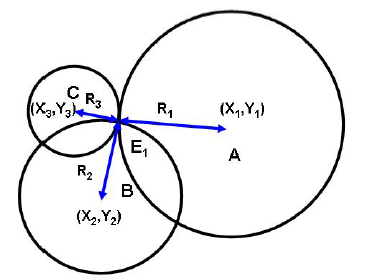
\includegraphics[scale=1]{graphics/triangulation.png}
		\caption{Triangulation\cite{Triangulation}}
		\label{fig:triangulation}
	\end{center}
\end{figure}

\subsubsection*{Angle of Arrival}
This category consists of approaches where the angle of the received signal is measured. The angle can be obtained by either having several antennas or being able to rotate a single antenna to find the direction at which the RSSI is strongest. With multiple angles of arrival it is possible to calculate a position based on the intersection of the euclidean vectors going through the antennas.

\subsubsection*{Location Patterning}
The location patterning category sets out to measure the connectivity patterns for a set of locations. The most common approach for this category is called WI-FI Fingerprinting. This method has an intial calibration phase, where the RSSI pattern for each point of interest is measured and stored in the system. When the signal strength from a device is received, it is then compared to the previously measured RSSI patterns. The point of interest with the most similar pattern is determined to be the position of the device. This means that a system using fingerprinting can not determine the exact position of a device, but rather calculates a probability that the device is located at a given point of interest\cite{fingerprint1}.

\subsection{Evaluation dimensions}
When evaluating indoor location services there are three dimensions that we can evaluate quality on: location precision, refresh rate and system latency. Location precision tells us about the location precision that the system affords. Refresh rate is the rate at which the location is updated, and as such how closely the most recent data is related to real-time data. System latency is a dimension describing the time it takes to perform the positioning calculations\cite{dimensions}. Depending on the usage of the system, the dimensions can be valued using a scale of importance, such as "High", "Medium" and "Low". Alternatively we can chose to look for systems with one or more dimensions below a set value. For instance, we have a desire to find a system with a location precision lower than the average precision for GPS which in 2014 was set to have four meters of inaccuracy \cite{gps_report}. 
\ofx{Should be cite buy cant compile when i change it}

The three dimensions are in no way constant for a system. For most systems, the hardware has a large influence on the dimensions. For instance, location precision for Triangulation is severely diminished if the environment lacks access points. Refresh rate depends on how often mobile devices communicate with the network and system latency can be impacted by a large amount of noise on the WI-FI channels. \Cref{tab:evaluating_approaches} shows the influences for the four tracking approach categories for each evaluation dimension. The system latency of a system entirely depends on the software, hardware and communication protocols used.

\begin{table}[]
\centering
\begin{tabular}{|l|p{4cm}|p{4cm}|p{3.5cm}|}
\hline
                    & Location Precision                 & Refresh Rate             & System Latency    \\ \hline
Cell of Origin      & Within cells                       & On checkpoint register   & Depends on system \\ \hline
Distance            & Depends on amount of access points & When device communicates & Depends on system \\ \hline
Angle of Arrival    & Depends on amount of antennas      & When device communicates & Depends on system \\ \hline
Location Patterning & Depends on calibration phase       & When device communicates & Depends on system \\ \hline
\end{tabular}
\caption{Evaluation dimension in relation to the four tracking approaches}
\label{tab:evaluating_approaches}
\end{table}

\subsection{Technologies}
In this section we examine some systems using different tracking approaches that aStep can use to integrate indoor positioning.

Zonith Indoor Positioning System is a system that uses the cell of origin approach. As mentioned in \cref{sec:tracking_approach}, this technique requires auxiliary hardware. Zonith offers Bluetooth Beacons, which serve as checkpoint nodes, and allow for any device with Bluetooth to be discovered and tracked\cite{zonith}.  Because of the nature of the approach we expect the location precision is excellent at the moment the device is registered, and the quality of the data decays as it ages. However, the most recent registration of a device is an approximation of its location, at best it tells us what room the device is in.

Redpin is an open source indoor positioning system that uses location patterning. The system requires a calibration phase, where the connectivity fingerprint of different key locations is measured. A users location is calculated on request, and, with enough fingerprint meaasurements, the system will be able to provide the user with at least room-level accuracy\cite{redpin}. Location precision is as such dependent on the calibration phase, but is expected to be better than a cell of origin approach. 

Google have also developed their own positioning system. They have made indoor navigation and tracking possible trough their Indoor Maps project \cite{IPSoverGPS}, which lets users map a building by uploading a floor plan of said building. After the floor plan has been accepted, the system will request information about the location of the WI-FI access points in the building\cite{googleindoormaps}. A user can then see their own location on Google maps at any time. Google have been very secretive in regards to what tracking approach they use, as such it is difficult to evaluate the technology.

Cisco have developed a location-aware wireless network system, Cisco Mobility Services Engine (MSE), which utilises WI-FI triangulation\cite{CiscoTri}. MSE makes it possible for Cisco to track the location of up to 25000 network devices at once, regardless of whether the devices are connected to the network. Using the RSSI data from the access points, the Cisco controller calculates distance and compares time of arrival to perform a triangulation and obtain a position\cite{ciscoMSE}.
The building is modelled by the use of an outline of the floor plan. The image is converted to a coordinate system that is placed on top of the model, which is then supplied with the positions of the static access points in the building. With this information it is possible to get the relative position of any device in relation to the origin of the coordinate system. It is these relative positions that are used to track wireless devices.
Cisco claim to have a location precision of less than a meter, refresh rate of 10-120 updates per minute and a system latency of 2-4 seconds\cite{dimensions}. 

\subsection{Choice of Technology}\label{subsec:cisco}
We have presented four technologies using different tracking approaches. We impose two requirements for the technology. First, we largely prefer a system with an accurate location precision. In practice this means being able to position people within rooms, as indoor environments can differ greatly in room size. For instance, an airport is difficult to partition into rooms, as it normally exhibits very open spaces. Secondly, we wish to harvest as much data, in terms of positions, as possible. This allows for predictions on crowd movements, path-finding to circumvent crowded areas and analysing typical movement in a building. 

Our first requirement excludes the Zonith Indoor Positioning System. To accommodate the second requirement, we examine the obtainable data from the systems. Redpin affords the possibility to request the position of a single device. Given that it is open source, it will be possible to alter the system in such a way that all devices on the network is provided. Google Indoor Maps only allows requesting a single user. Cisco MSE has the functionality to provide a list of devices registered along with their most recent position.

There are several arguments pointing towards Cisco MSE rather than Redpin. First and foremost, Cisco MSE is in comparison a lot more convenient, as it already affords the desired functionality and requires substantially less set-up time. Secondly, the amount of documentation for Cisco MSE far outweighs what little documentation there is for Redpin. Cisco MSE is a commercial system, and is therefore updated regularly. As of 7/3/2016, Redpin had its most recent update in May 2013. As a consequence of these arguments we chose to integrate Cisco MSE as the indoor positioning system for aStep.

Aalborg University uses the standard version of Cisco MSE to position devices on their network. We plan on using the data available from this system as dummy data for the aStep project.
%Alternative IPS 
%se what we did in cisco 
\section{Permission} \label{sec:permission}
By using MSE it is possible to acquire and store peoples unique MAC address and use this to track them. It is illegal to do so without the individuals acceptance and it is as such necessary to accommodate this regulation when designing the system \cite{TrafficIlligal}.
There have been several trials in Denmark as a consequence of this regulation. A Traffic system has recorded passerbys by registrating the WI-FI signal emitted from their smart phones. This was done with sensors registrating the unique MAC address, which was then hashed and re-hashed in the sensors before being stored. Despite the attempt at obfuscating the users \cite{TrafficIlligal}, it is illegal according to the \textit{Directive on privacy and electronic communications} article 5(3) \cite{CookieDirective} which can be seen in the following quote,

\begin{quote}
\textit{'Member States shall ensure that the use of electronic communications networks to store information or to gain access to information stored in the terminal equipment of a subscriber or user is only allowed on condition that the subscriber or user concerned is provided with clear and comprehensive information...'}
\end{quote}

However, the Danish Business Authority's conclusion was that the system did not fit in \textit{Directive on privacy and electronic communications} due to the end user being unidentifiable \cite{TrafficOK} as described by article 3(1) \cite{CookieDirective}. No sanction was inflicted for this case, however, this illustrates the necessity to obfuscate personal sensitive information.

%http://eur-lex.europa.eu/legal-content/DA/TXT/PDF/?uri=CELEX:31995L0046&from=da
To ensure no such debates are raised in relation to this project, it will be necessary to differ between those who have given their permission to store person sensitive data and those who have not. By differentiating between the two it will be possible to obfuscate and remove personal data, such as MAC addresses, for individuals who has not given their acceptance.

We will use the term person sensitive data when referring to data that can be used to identify a person. 
\section(security)
This sections goal is to secure the data that will be send from the Cisco system to the database described in figure \jfx{ref til figuren i cisco}. The alternative methods will be explored in this section and chosen a methods to implement.

\subsection{Encryption}
Encryption is used to ensured that only the intended people will be able to extract the data, this is not entirely correct, because unwanted people will still be able to see the data and would in practice be able to decrypt it. This can be semi-counteracted by increasing the bit encryption, which will exponentially increase the time take to brute force the encryption. So when security is discussed there are to impotent factor in play,
\section{Using Cisco}\label{sec:cisco_usage}
The Cisco localisation and positioning system is already in use at Aalborg University. To be able to use the information from the system, we had a meeting with the administrator, during which he raised concerns for privacy, because of the legality of storing person sensitive data, as mentioned in \cref{sec:permission}. Furthermore he wishes to be able to provide the location data to future student projects with ease. To accommodate this, it has been asked of us to build and deploy an intermediate service with the goal of obfuscating sensitive personal data, such as MAC-addresses and user names. This service is intended to duplicate the functionality of the Cisco MSE RESTful API, such that the service acts as a transparent proxy. This is achieved by creating an intermediate RESTful service, that simply redirects requests and processes the response before sending it back to the initial requester, as illustrated on \cref{fig:cisco_usage}.

\begin{figure}[ht]
	\begin{center}
	\includegraphics[scale=0.9]{graphics/cisco_usage.png}
	\caption{Cisco usage}
	\label{fig:cisco_usage}
	\end{center} 
\end{figure}

A RESTful service typically communicates using the HTTP or HTTPS protocols, and functions by receiving requests for specific data resources, called Uniform Resource Identifiers (URIs) to which it responds by sending the requested data. As an example we can send a HTTPS GET request to 64.103.26.61, which is a Cisco MSE test server, with the URI "/api/contextaware/v1/location/clients" and, given that we supply the correct user name and password, receive a string of data corresponding to the type of request \cite{restful_oracle}.

To create a transparent RESTful service that duplicates the functionality of the Cisco RESTful API, we need to make use of the same URIs as the Cisco API\cite{cisco_mse_api}. This is done with the use of the Jersey Java library, which affords the possibility of creating a HTTP server and specifying what URIs are available for a client to request.

\begin{lstlisting}[caption={Adding a URI},label={lst:context_code},language=inc_Java]
server.createContext("/api/contextaware/v1/location/clients", httpExchange -> {
            if (VerifyConnection(httpExchange) == false){
                return;
            }

            String response = CollectAllClients(username, password, ciscoIp);
            httpExchange.sendResponseHeaders(200, response.length());
            OutputStream os = httpExchange.getResponseBody();
            os.write(response.getBytes(Charset.forName("UTF-8")));
            os.close();
        });
\end{lstlisting}
The code example shown on \cref{lst:context_code} shows an example of how to specify a URI. The createContext() method on line 1 takes two parameters: a string for the URI and an anonymous function implementing an interface. The anonymous function taking up the rest of the example dictates what actions are performed once a connection is established. In this case some verification is performed immediately after the function call, to authenticate the user. A response is generated based on the URI; on line 4 we retrieve all clients from Cisco using the ColletAllClients() function, which also performs the task of obfuscating necessary information. The list of clients is then written though an OutputStream to the requester, as seen on lines 8 and 9. The anonymous function terminates as the OutputStream is closed, which also serves as a termination of the HTTP connection. 

In order to accommodate the privacy concern, we implement some simple methods to obfuscate MAC-address and user name, one of which can be seen in \cref{lst:obfuscating_mac}. It might be the case that users allow for us to store their personal information, and as such we will have to make a check to see if this has been allowed. To store this information we use a TreeSet, which guarantees $log(n)$ time cost for adding, deleting and searching \cite{treeset}. On line 2 we obtain the MAC-address of the user, which is used on line 3 to perform a search in the TreeSet. If search returns empty we obfuscate the MAC-address, as seen on line 4. This is done in a similar way for the user name.

\begin{lstlisting}[caption={Obfuscating mac-address},label={lst:obfuscating_mac},language=inc_Java]
Private static Client ObfuscateMacAddress(Client singleClient) {
    String oldMacAddress = singleClient.getWirelessClientLocation().getMacAddress();
    if (!watchList.contains(oldMacAddress)) {
        singleClient.getWirelessClientLocation().setMacAddress(obfuscatedAddress);
    }
    return singleClient;
}
\end{lstlisting}

\subsection{System hierarchy}
With this code it is possible to create an intermediate service for the Cisco MSE RESTful service, that intercepts the response and obfuscates certain information. To use this service, a client needs to know the IP address and a login for the intermediate service. To automate the requests and create a flow of data from the Cisco systems to the aStep database, we will have to build and implement a client that fetches data at an interval. The scope of the project is beyond Aalborg University, and as such we want to integrate more than a single Cisco MSE system. 

\begin{figure}[ht]
	\begin{center}
	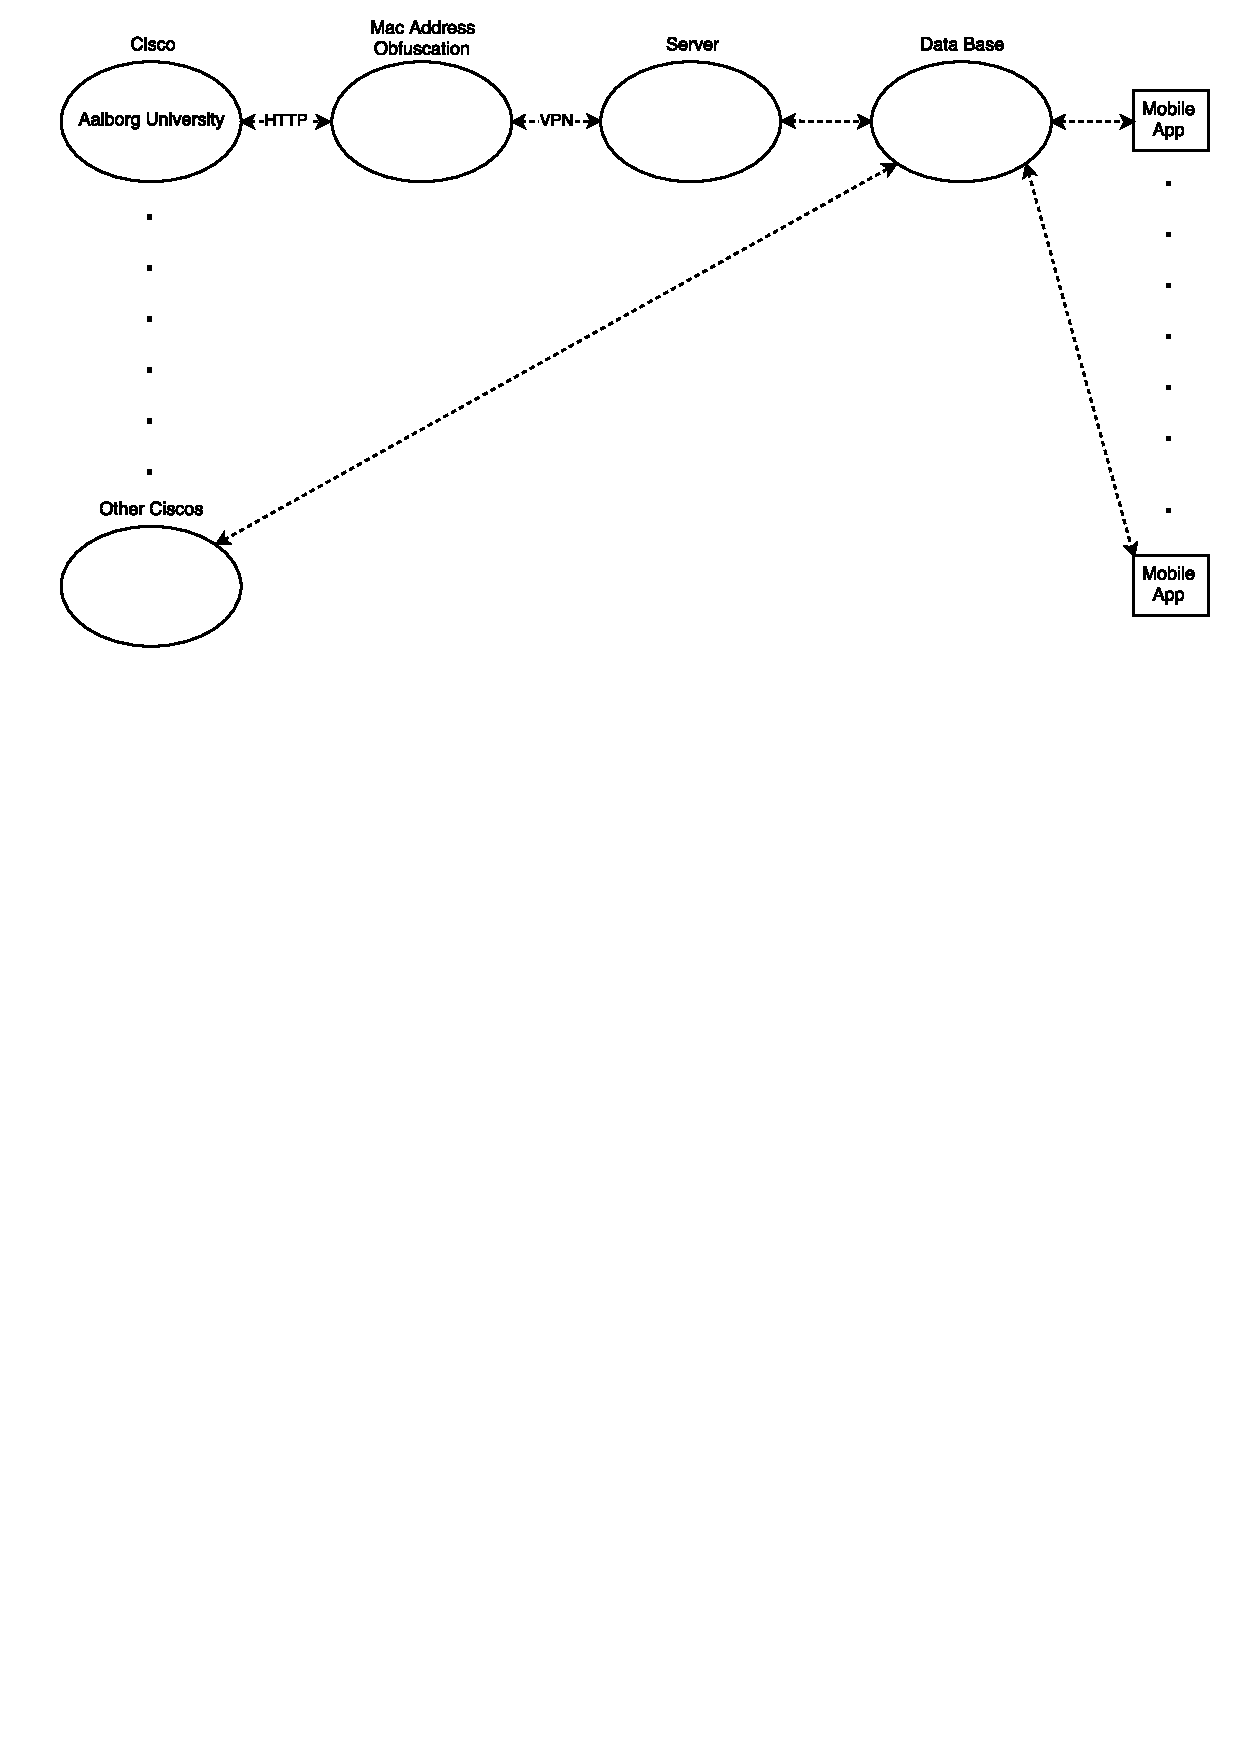
\includegraphics[scale=0.5]{graphics/ciscoSmall.pdf}
	\caption{Cisco systems}
	\label{fig:cisco_systems}
	\end{center} 
\end{figure}
\Cref{fig:cisco_systems} shows how the information flow is intended. The client connecting to the Cisco services can function as a server that requests data from all Cisco services that we have access to. Alternatively, a server can be implemented for each Cisco service. However, this solution has several downsides. First, it means corporations supplying the aStep project with information will have to have hardware running the server, which requires maintenance. Second, this solution is not scalable. The server running the aStep database will potentially be overloaded, as it has to handle each individual Cisco system sending information. As more Cisco systems are added, there will be less time to process received data. An alternative approach is to have the aStep database server request data, however, with an increase in connected Cisco systems, the interval at which we receive new information from a given system also increases. The optimal solution to this issue is to create a hierarchy of servers, such that the database server only receives data from a constant amount of intermediate servers, each of which also receive information from an amount of sources. During the start up of the aStep project we have access to a single Cisco MSE system, and as such we will not focus on building this hierarchy. However, as the project grows and additional Cisco systems are integrated, it will eventually become a necessity.  

\section{Sprint Evaluation}
To conclude on the first sprint, we have explored different methods and technologies to perform indoor positioning. Furthermore we have described certain issues related to person sensitive data, and finally we developed an initial design of a RESTful service to operate as an intermediate service for Cisco MSE. 

As such the goals for the first sprint have been fulfilled.
\chapter{Sprint 2}

One chapter per development cycle (i.e., one chapter per sprint) performed in the project documenting the analysis, design, refactoring, implementation and test performed in that cycle.

Each cycle may contain more or less of each of these elements.
This chapter covers the “design of an application that handles a substantial part of this” and “development of a program that realizes the design”

\chapter{Sprint 3}\label{cha:sprint3}
This sprint aims to explore the possibilities of building our own tracking system as well as updating the restful intermediate service. Furthermore, we will examine our systems in regards to the aspect of security. 
\section{Building our own tracking system using routers and hotspots}
This section will include the advancements made in building and gathering of information about using routers and hotspots to make our own ILBS, a list of objectives can be seen below. The goal for this is enabling us to calculate the position of ourself in geographical coordinates and compare them to the coordinate provided by Cisco.

\begin{itemize}
	\item Equipment Requirements
	\item Test Capabilities of the Router 
	\item Test Capabilities of the Access Points\ofx{is this all?}
\end{itemize}

An overview of the entire system can be seen in \cref{fig:OwnSetup}. One router and four access points are set up in our group rooms, such that it covers three group rooms.
\begin{figure}[H]
	\centering
	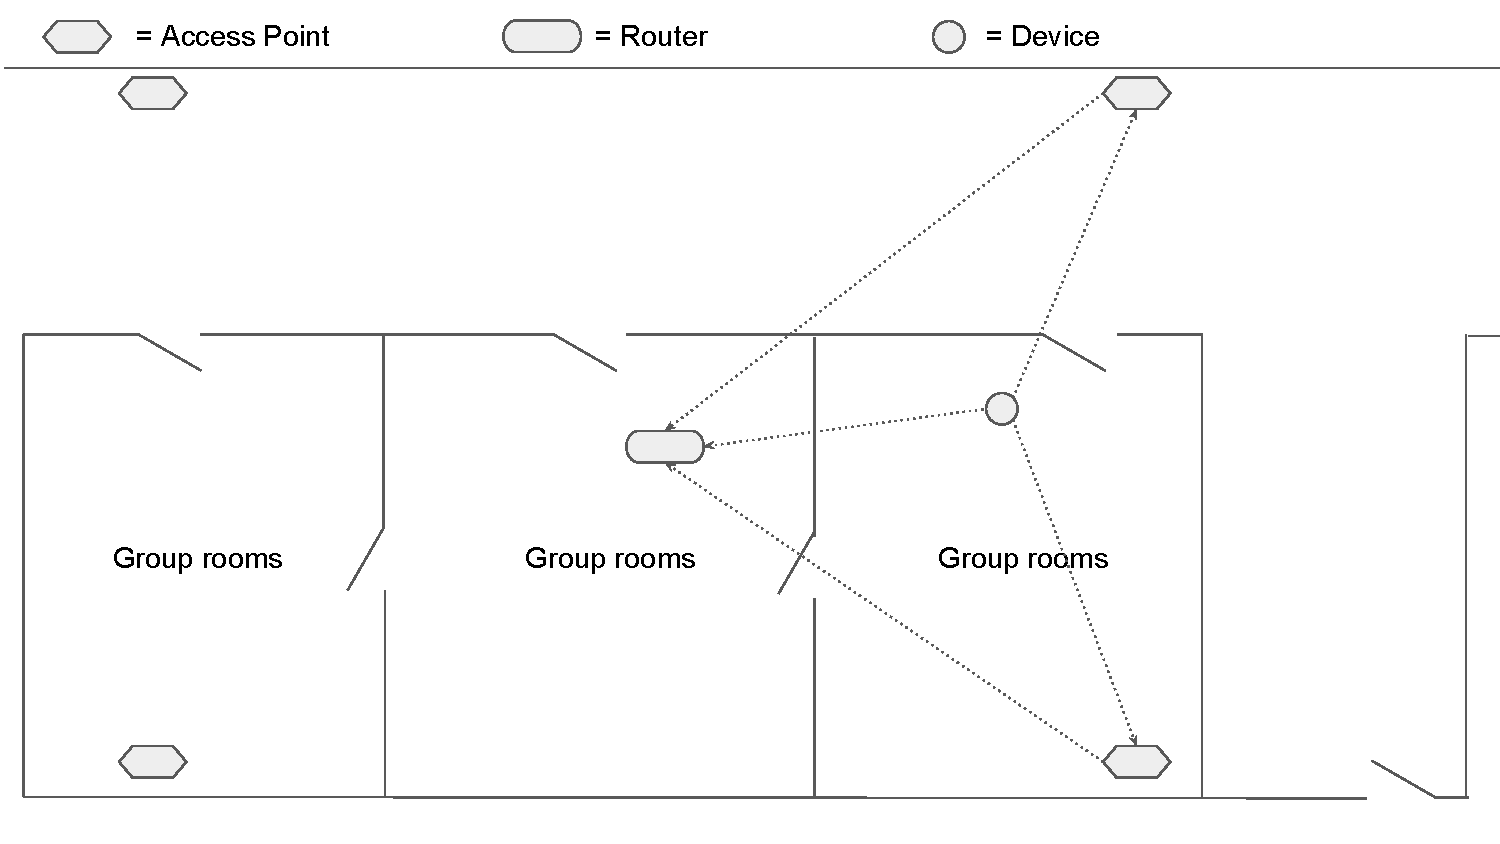
\includegraphics[scale=0.5]{graphics/Router-AccessPoint_Setup.pdf}
	\label{fig:OwnSetup}
	\caption{Illustration of how a positioning system can be set up, using routers and access point that can track devices.}
\end{figure}

\subsection*{Equipment Requirements}
The initial requirements for the equipment, is a wireless antenna capable of supporting 2.4 GHz and optionally 5 GHz. It would be advantageously if we set up two different ILBS for the sake of comparison. We decided to buy two brands allowing us to analyse at least two ILBS and thus conclude which of the systems performed best, based on the criteria describe in section \ref{sec:monitoring}.

Based on the above requirement we found two brands, Ubiquiti and D-link which in comparison is considered the cheaper brand. We ordered one router, two expensive and five cheap access points of each brand.

\subsection*{Access point positioning}\ofx{we may want to move this?}
Cisco\cite{access_point_placement} have guidelines for how to place the access points in order to get the best coverage for your system. They recommend that there are placed an access point in each corner of the building and some along the perimeter, in addition if the building is large enough there should be placed some within the perimeter that can form a sub-perimeter inside which there may be additional access points, this is illustrated in \cref{access_placement} on which the red circles are access points. This means the perimeter established by the outer most access points should encapsulate the entire floor. Everything on this perimeter is called the \textit{hull}\cite{access_point_placement}.

Each access point should be place 50-70 feet away from each other in order to get a high precision without a lot of unnecessary overlap\cite{access_point_range}.
 
The placement of the access points in \cref{fig:OwnSetup} is based on this design. As it can be seen they are placed in a square to symbolize corners and the router in the middle, in our small system.

\begin{figure}[H]
	\centering
	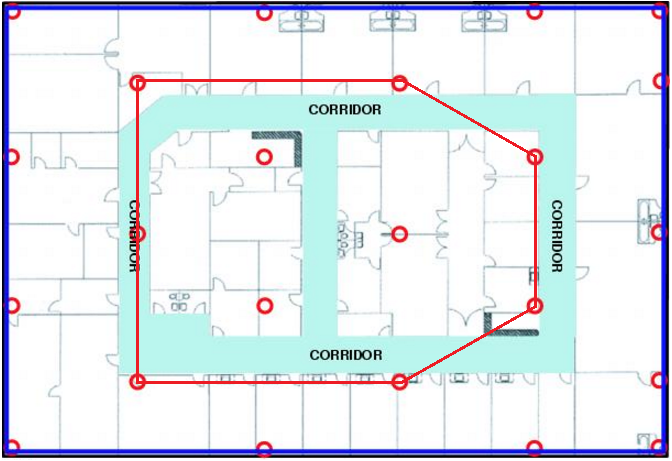
\includegraphics[scale=0.5]{graphics/access_placement.png}
	\label{fig:access_placement}
	\caption{Illustration of how access points should be placed.}
\end{figure}

\subsection*{Test Capabilities of the Equipment}
We tested the Ibiquiti equipment, with the original firmware. At first glance we are able to get transmission(TX) and receive(RX) signals of connected devices, unfortunately we do not receive the signals from devices not connected to the router. It was attempted to use the routers terminal which did not yield any results due to restricted access.

This caused us to research custom firmware for the router. By installing new firmware on the router we will be able to get root access to the router and thereby manipulate it at a lower level than the routers original firmware allows, this is necessary if we are to capture every receive signal the router gets.

We did find a custom firmware for Ibiquiti, however not for D-link. The searched sites were: openwrt.org{cite?}, polarcloud.com\ofx{cite?}, dd-wrt.com, gargolye-router.com\ofx{cite?}, librecmc.org\ofx{cite?} and wrtrouters.com\ofx{cite?}. These sites covers thousands of routers and the fact that we were not able to find a custom firmware for D-link might be because that the particular model we ordered\ofx{something is missing} because other routers from the same brand is supported. No conclusion was found, to why it is not covered on any of the websites.

We ended up utilizing the openwrt because it supports our Ibiquiti router and allows us to gain root access and execute programs. With the new custom firmware installed we have about 8Mb of memory left on the router, this put some limitations to which language we can use, our first attempt is to use a version of python called mini-python that dose not exceed the memory limit.

A program is constructed allowing us to listen on different types of networks such as LAN and WAN, this is done using the socket library. We were however not able to import the socket library which was required, to run our program on the router.
\section{Intermediate Server Update}\label{sec:proxy_update1}
We plan on implementing an update to the intermediate server that is used to communicate with Aalborg University's MSE. This update is a consequence of MSE being updated to support geographic coordinates. The update is planned to remove a bug causing loss of data during conversion between different data formats. This section covers the motivation for the following changes in the update:

\begin{itemize}
\item Resolved loss of data during conversion
\item Obfuscates new data acquired as a result of aforementioned change
\item The service no longer stops if it loses its connection with MSE
\item Now checks if MSE is online, and whether the right account information is received, at start-up
\item Supports paging
\end{itemize}

\subsection{Loss of Data}
Geographical coordinates are now supported by MSE, thanks to the MSE administrator at Aalborg University. To perform obfuscation of personal sensitive data, we can convert the returned string to classes containing all information in its member variables. With this method we can easily perform obfuscation of the data we are disallowed to keep by editing the fields corresponding to the personal sensitive data.

This method utilizes a library developed by Google called gson \cite{gson}, which affords the ability to convert strings of the JSON format to a Java class and vice versa. We can acquire the classes by using an online tool called jsonschema2pojo \cite{jsonschematwopojo}, that analyses JSON strings and automatically generates classes with corresponding fields.

Initially, the generated classes did not contain fields for the global coordinates, as they were based on the response string from a version of MSE where this feature was disabled. This would not be a problem for a single conversion, as the generated classes have a field called \textit{additionalProperties}, which contains additional information that could store the coordinates. However, in order to preserve the transparency of the intermediate server, we wish to perform a conversion back to JSON in order to maintain the external illusion of this intermediate server being an MSE service.

Performing several conversions results in a loss of data, as any information in the additionalProperties field is lost. To avoid this data loss, we can re-generate the classes using a JSON string with the appropriate information. Alternatively, we could perform a string search for specific keywords in the JSON string, which we would then obfuscate. However, search and replace in strings is undesirable, in particular because the JSON string often is more than a million characters long. The class of strings in Java is immutable, meaning any changes to a string variable results in new memory being allocated and the modified content of the old memory location copied over. Performing replacements in a large string is very expensive, and it is as such desirable to perform the aforementioned class conversions. 

As a result of the update we now receive specific information that were previously unattainable through the MSE developer test system. This information includes personal sensitive data, which is now being obfuscated when necessary needed. 

\subsection{Connectivity with MSE}
After the initial deployment of the service we experienced downtime as a result of MSE being under maintenance. This was an unexpected event, and as such the program reacted in an unforeseen fashion. Part of the update integrates elements from the client, described in \ref{sec:fetch_data}, in an effort to increase robustness and as such uptime of the service. As a result, the service now sends an initial request to MSE, to confirm the MSE IP address and account info. Furthermore, the service is able to handle MSE being unresponsive.

\subsection{Paging}
When requesting all clients from MSE the response is partitioned into pages. Each page contains a certain amount of entries, as defined in the request. If this is not defined in the request, a default of 5000 entries per page is used. 

Initially we were not aware of this feature, as the MSE test service never made use of paging. As a result, we would only receive the first page of information, missing out on thousands of entries. This update aims to implement a correction, which will enable the use of paging in a request. After this update it is possible to explicitly state which page is requested, whenever a request is sent.

During this sprint we examined the possibility of building a small tracking system with only a tree and our bare hands. We deployed an update for the intermediate service communicating with MSE, fixing several issues and creating support for global coordinates. 
\chapter{Sprint 4}
This is the last sprint and will be dedicated to implementing the last features discovered in sprint 3 and improved the overall code standard, it includes hashing password and mac-addresses and enabling HTTPS on our server. Additionally a section will be made dedicate to future developer of aSTEP, to make it easier to get up to speed.

\section{Catching Up - Introduction to Using Our Project}\label{sec:catchup}
This section will contain guides describing what elements to be aware of in the system and how to perform different tasks for maintenance and further development. We write this section to ease the change of ownership, such that the new owners can avoid problems we experienced and spent time resolving. 

\subsection*{Transfering a Program to the Virtual Server}
We recommend testing new changes as thoroughly as possible before going through this as this process is tiresome to do a lot. Before doing this you need to contact the Cisco MSE administrator of AAU and ask for passwords for the virtual proxy server and MSE. The current administrator is Per Mejdal Rasmussen from ITS. Let him know that you are continuing development of the proxy server connecting us to MSE.

Sending the Java program to the virtual intermediate server:
\begin{itemize}
\item 1) Compile the artifact such that you get a .jar executable file. Test it on your own system by running "java -jar FILEPATH" on your own system.
\item 2) Upload the .jar to a website you can download from. We used dropbox. Get the shared link on Dropbox for the file.
\item 3) Open putty and connect to "sshgw.aau.dk".
\item 4) Login with your usual moodle account.
\item 5) ssh to root@mon-mse-proxy.srv.aau.dk with the command "ssh root@mon-mse-proxy.srv.aau.dk".
\item 6) Login with password - this is something you request from the MSE administrator.
\item 7) Navigate to the home directory. This directory contains directories for current and previous versions of the program. Move current version and other files to another folder. 
\item 8) Check if any screen session is active with "screen -ls". If this is the case, kill the process with "killall screen".
\item 9) Download the .jar file with the command: wget -O MSEproxy.jar "DROPBOXURL" 
\item 9a) Make sure to put a download=1 at the end of the url if using Dropbox.
\item 10) See that you have the file in the directory, run the program and make sure it runs correctly. Command to run the program is on step 14.
\item 11) Change user to MSE with the command "su - MSE -s /bin/sh".
\item 12) Type "script /dev/null".
\item 13) Check if any screen session is active with "screen -ls". If this is the case, kill the process with "killall screen".
\item 14) Navigate to home folder containing .jar and run the program with command: "screen java -jar MSEproxy.jar https://172.18.37.70 mse-proxy PW", where PW is replaced by the password given by the MSE administrator.
\item 15) If all is well you get a message saying the server is up and running on some IP. This is the IP you connect to. The port is important as well, it has to be 8080.
\item 16) Detach from the screen by holding down CTRL+a+d.
\end{itemize}

\subsection*{IntelliJ Debug Configurations}
When further developing the project it is useful to share the debug configurations, such that the project setup only has to be done on one computer. In IntelliJ, open the Edit Configurations screen and tick the shared box. This creates a folder in the .idea project folder called runConfigurations, which can be shared. When opening the project, IntelliJ will automatically detect existing debug configurations in this folder.

\subsection*{Projects under Indoor Repository}
The Indoor (ID) Gitlab repository contains several IntelliJ projects. The projects are called: testingPrograms, RestfulMSE, indoorLibrary, indoorCore. Additionally you will be able to find a JavaDocs folder containing code documentation.

\begin{itemize}
\item Testingprograms is a simple project used to debug a RESTful service. This can equally be done with a tool in IntelliJ (under Tools -> Test RESTful Web Service), however, we do not advice this as everything has to be input each time it is to be tested. Testingprograms contains very little functionality and is only meant to be used for HTTP get calls.
\item RestfulMSE is the project for the intermediate proxy server. 
\item Indoorlibrary is a static library containing much of the functionality used by our programs. We early on realised that the two systems are alike in many ways, and would have to afford the same functionality. As a consequence we decided to make a library to use across several projects, to avoid duplicate code. 
\item IndoorCore contains the code for the client service. 
\end{itemize} 

\subsection*{First Time Opening the Program}
This is a step guide to setup the IntelliJ IDE with the project.


\section{Client Server}

\subsection*{Enabling HTTPS}

\subsection*{MSE Error Handling}\ofx{maybe give another title}
It may occur that MSE is not running if this is the case it should be communicated to the user. As of now, it is possible to visit a restful service communicating if MSE is running or not. This however may seem insufficient for a user, especially if the user is receiving continuous data. Therefore the client should be able to communicate if it is not getting any data from the intermediate server. By doing so the user would get a message as soon as MSE stops working.
\section{Intermediate server update}

\subsection*{Logging}
The intermediate server utilizes Log4j\cite{log4j} to log error messages when it is executing. These messages are stored in a log file saved locally with the server which can be accessed and read. The log only concerns errors and alike, but we believe it would be beneficial to have an additional log the records other messages as well. We would like to log requests to the server by their time, request type and request sender. That information can be used to debug potential errors and to analyse the connectivity history. 






\subsubsection*{Password}


\section{Code refactoring}
In this section we describe the changes made to the code in the fourth sprint.

Since this project will be developed on by other people in the future, we find it essential to improve the code as must in terms of readability, further detail will be discriped in the sub section "Code Improvement"

\subsection*{Hashing of MAC-Address}
Due to a request from the Heatmap group, to be able to track people by some unique value, we have elected to hash the MAC-Address rather than obfuscate with "OBFUSCATED". In \cref{sec:secure}, we explored the possibility of doing so, by using Javas hashCode(), which is implemented in the String library. However, hashCode() returns a string consisting of only integers, which gives a higher risk of having overlap when hashing. Instead we chose to use the Guava-19 library which returns a much longer value consisting of both numbers and letters. By doing so it allows for hashed MAC-Addresses to contain letters making it more difficult to brute-force. The salt applied is a random string that is changed every twelve hour. 

The applied function can be seen in \cref{lst:ourhash} where in line 1 the MAC-Address is concatenated with the randomly generated salt-value. In line two the new string is hashed using Guava-19's sha256. In line 4 the MAC-Address is set to the hashed value. The hashed value is 64 signs long and contain both letters and numbers.

\begin{lstlisting}[caption={Hashing a MAC-Address},label={lst:ourhash},language=inc_Java]
oldMacAddress = oldMacAddress + salt;
String hash = Hashing.sha256().hashString(oldMacAddress, 
	StandardCharsets.UTF_8).toString();
item.setMacAddress(hash);
\end{lstlisting}

\subsection*{Adding servers to client}

\subsection*{Code Improvement}
By using the IntelliJ IDEA we are able to use one of the build-in tools "Inspect code" to analyse the code and come with suggestions, this is done for the project; RESTsw6 and the two libraries; indoorCore and indoorLibrary. When inspecting code, we receive suggestion to Class structure for moving some of the global variable into a sub scoops were they are used to hide information. Declaration redundancy concerns variable access level and making variable final, This also includes empty methods and redundant parameters. Imports handles unused packages, Probable bugs finds constants conceals as variables and Spelling question the naming of variables. Important to remember it only suggestion, because inspect code is not already able to see how the class or method is used, this will result in unrealistic suggestions that are more likely to break the code.


\section*{Security}
To increase security we decided from sprint 3 evaluation to hash the MAC addresses and get switch from http to https on the intermediate server.

\subsection*{Hashing of MAC Address}
Due to a request from the Heatmap group, to be able to track people by some unique value, we have elected to hash the MAC address rather than obfuscate with "OBFUSCATED". In \cref{sec:secure}, we explored the possibility of doing so, by using Javas hashCode(), which is implemented in the String library. However, hashCode() returns a string consisting of only integers, which gives a higher risk of having overlap when hashing. Instead we chose to use the Guava-19 library which returns a much longer value consisting of both numbers and letters. By doing so it allows for hashed MAC addresses to contain letters making it more difficult to brute-force. The salt applied is a random string that is changed every twelve hour. 

\begin{lstlisting}[caption={Hashing a MAC address},label={lst:ourhash},language=inc_Java]
oldMacAddress = oldMacAddress + salt;
String hash = Hashing.sha256().hashString(oldMacAddress, 
StandardCharsets.UTF_8).toString();
item.setMacAddress(hash);
\end{lstlisting}

The applied function can be seen in \cref{lst:ourhash} where in line 1 the MAC address is concatenated with the randomly generated salt-value. In line two the new string is hashed using Guava-19's sha256. In line 4 the MAC address is set to the hashed value. The hashed value is 64 signs long and contain both letters and numbers.

\subsection*{Enable HTTPS on the Intermediate Server}
Using "lets encrypt" we can enable https, this was done to the aSTEP server, so we contacted one of the people that ended up doing to final work. He said it took about 3 weeks and the reason why it took so long was because of them not being able to open port and setup a domain which is required for lets encrypt. So we will not be able to do this task duo to our deadline. A section under future work will explain this task to accommodate, because it seen as essential to reach the minimum concerning security

\section{Sprint 4 review}

%%%% COLLABORATION %%%%
\chapter{Collaborations}
a quote from the report guidelines for aSTEP\cite{guidelines}: 
\begin{quotation}
	At least two topic focused chapters describing common activities performed with at least one (maximum three) other group (not the same for each chapter). These chapters can be written together with other groups such that they are identical in the different reports. These chapters should mainly be focus on the final state of affairs and not the steps along the way. They should be the ideal starting point for new developers to continue the development on the system. It is emphasized that a project cannot cover all of the topics listed in the study regulation list and that this should not be penalized. These chapters should be focused on relevant problems in the project, such as:
	\begin{itemize}
		\item Project management
		\item Requirements analysis
		\item Requirements management
		\item Prototyping
		\item Databases
		\item System architecture, common class diagrams
		\item Usability; usability design, usability test
		\item Test and verification; integration test, acceptance test, regression testing, protocol verification
	\end{itemize}
\end{quotation}

This means we need to make at least two collaborations with other aSTEP groups.

\section{GitLab}
At the aSTEP meeting that took place at 17.02.2016 it was decided that a few people across the groups should take responsibility for maintaining the GitLab server, to ensure that GitLab is running as decried, without causing any of the groups, assigned to the aSTEP project, problems. Two members of this group volunteered for this task. 
%The purpose of the following section is to describe the work that we have done related to GitLab. 
The formed GitLab group used Slack to communicate and assign tasks within the group. The different tasks related to GitLab was assigned to the members of the GitLab group.

\subsection{GitLab Update}
The first task assigned to our group was to update GitLab which is running on the semesters virtual server, hence refereed to as the aSTEP server. It was agreed that the best approach would be to install a virtual server on a computer, to emulate the GitLab update. This was done to ensure that in case the update would fail it could not cause problems to the aSTEP server.
%The magnitude of this task involves installing a virtual server on a computer to emulate the GitLab update to ensure that if it fails, it will not cause problems to the aSTEP server which is running the actual GitLab service. 
The reason for updating GitLab is in order to increase performance, which have been achieved for builds as well as runners, push and pull. 

To do so the program VirtualBox \cite{vbox} was used to emulate an Ubuntu Server operation system, where the GitLab service was installed. In addition PuTTY \cite{putty} is used to allow connection and communication with the aSTEP server.

In order to install a 64-bit architecture one must; turn on Intel (R) Virtualization Technology and Intel (R) VT-d Feature in Basic Input Output System (BIOS). Then disable Hyper-V in Windows Features, restart the machine and updated the setting. VirtualBox will now show the option for 64-bit. 
GitLab is now ready to be installed on the test machine by following the guide from GitLab's website \cite{gitlab_guide}.

%The installation process have an architectural conflict as GitLab runs on a 64-bit architecture and the standard configuration of VirtualBox on the test machine only shows the option for installing 32-bit systems. This is problematic as the update will fail if the version is 32-bit. It is possible to allow the 64-bit option to be displayed by changing the following setting on the test machine; turn on Intel (R) Virtualization Technology and Intel (R) VT-d Feature in Basic Input Output System (BIOS). Then disable Hyper-V in Windows Features, restart the machine and updated the setting. VirtualBox will now show the option for 64-bit. 

%GitLab is now ready to be installed on the test machine by following the guide from GitLab's website \cite{gitlab_guide}.

To test the update a backup must be extracted from the aSTEP server. %To extract a backup and upload it to the testing server a sub program of PuTTY, called pscp, will be used. This allows extraction from the aSTEP server and the uploading of files to the test machine.
When the backup is extracted the next step is then to update GitLab with the new version. GitLab developers have incorporated some measures to ensure that the GitLab servers will not lose data even if an update fails. This is done automatic by creating a backup before installing and detailing the process in a log if anything went wrong, along with a set of solutions to the possible problems.

After this was done a Wiki page was created in the shared GitLab Wiki that would help future semesters in updating GitLab if necessary. The whole process of setting up a virtual test server will not be descried in the Wiki. It was deemed not to be necessary since GitLab have an automatic backup feature.

\subsection{GitLab Merge}
\ofx{Can you write an initial section on this Anders?}

\subsection{GitLab group work}
What were the other members of the GitLab group doing? 
build
runner

%Anders Merge request stuff, runners
%Rune overall håndtering, runners
%Alex committer en fandens meget!


%%%% EXPERIENCE %%%%
\chapter{Experience}
%A chapter documenting the experiences gained from working in a multi-project. Reflections and knowledge to be passed on to future students.
%Summary, Reflections, suggestions for next year students
\section{Working in a Multi-Project}
When working in a multi-project we are encountered with a set of different challenges compared to working in the traditional format, which we are used to.
%TODO der skal nook være lidt mere intro her

\subsection{Organisation}
It is necessary to enforce an organisational structure to efficiently establish an overview of the project when collaborating with a large group of people. As described in \cref{subsec:supergroup_meetings}, we needed to know how far the different groups were with their separate parts of the project and what kind of problems they were facing. If one group could not make any serious progress because of some hindrance, it was important that the other groups were notified, in case they were depending on their work. We uncovered the vast majority of these problems by organising what resembles a Scrum stand up meeting, at the super-group meetings where every representative reported their individual project status. If a group had a problem they were unable to solve themselves, they could draw help from the other groups, or move some of their tasks to them. It should be noted that it was only project wide tasks that could be transferred, such as updating the GitLab server or implementing a logging system.

The super-group meetings were accompanied by smaller project wide meetings where a single specific topic would be discussed. For instance, a topic we discussed was regarding the type of license that would be applied to the project.

A set of tools were used in order to ensure efficient communication acrss the multi-prject. In addition to the aforementioned meetings, the individual groups would occasionally arrange private meetings, as described in \cref{subsec:small_meetings}. These kind of meetings would usually involve two groups with some representatives from both parties. In order to avoid disturbing other groups when planning an meeting, the appointment would be discussed by using the message web application Slack \cite{slack}. It was encouraged to be discrete when contacting other groups as multiple groups share the same group-rooms, and external disturbances had to be kept to a minimum. This was also the leading factor for why many of these meetings took place outside of the group-rooms.

\subsubsection*{What Could Have Been Done better}
There was still room for improvement, both project wide and group wise, as instances of miscommunication, distrust to others groups work and lack of access to general information were all things % Nogen der kan komme på noget bedre end "things"? \Anders
 which occurred during the project.

We faced a problem internally in the group which sprung out from how we handled the information we got from the supper-group meetings. We would usually send the same representative who had two major responsibilities: verifying that we had prepared what was asked from us to the next meeting and conveying the key points from the last meeting to the group. It would be better if the representative was chosen anew each time in order to avoid that it was only one from the group who had a good overview of the project. Another solution could be to arrange a short intern meeting in the group after each super-group meeting in order to check that everyone is up to date. It would have been beneficial to solve this issue as the consequence was that we would sometimes forget to have completed certain tasks before their deadlines or went against some of the decisions that had been made. It would be beneficial for the overall project teamwork and the individual group member's sense of involvement in it.

A weekly topic that recurred on super-group meetings was the status update from each group. It was problematic that some groups did not take this presentation seriously and would not mention the problems they were facing our leave out details that might could have been useful for the other groups. It also meant that other groups perceived them as being slow and unresponsive to the requests that were presented with, even if it was them unfit and they actually did what they could in order to keep up. Groups would delay some of their tasks because they thought that the other group would \textit{soon} finish the part that they were depending on, even though that it might could take entire weeks before the part were complete. This was frustrating for those whom depended on the completion of the tasks it meant that they sometimes would need to redesign parts of their solution, or worse, cancel further work as they would not have time to finish. \\
It would be better if all the groups took the status presentation seriously such that issues could be resolved earlier or entirely avoided. % Skal vi komme ind på hvorofr vi tror at de ikke sagde noget? Skal vi komme ind på hvordan man kan løse det i mere detalje? Jeg har nogle ideer til begge dele. \Anders


\subsection{Working Environment}
% Hvordan sørger mna for at holde et godt arbejdsmijø? Konflikthåndtering, møder(brydder ind), ansvar
When working with multiple teams, it becomes apparent that mutual respect between the groups are important to uphold a healthy working environment.

One method to uphold this environment have already been mentioned, group meetings and the planning of them, but there are other areas of which one can have a positive influence. One such area is


\subsection{Overall Opinion}
% Konklussion? 
\input{experience/summary}
\input{experience/reflection}

%%%% FUTURE WORK %%%%
\chapter{Future Work}
\label{Cha:Future_Work}
In this chapter we describe what we believe will be advantageously for future students to look into in order to improve and further the system. 
%This chapter list the aspect of Cisco system and Indoor location based service work, for future semesters.
We will here discuss security, potential development of our IPS and changes that could be made to our systems. 



\section{Data Flow from Cisco to the Database}\label{sec:data_flow}
\begin{figure}[ht]
	\begin{center}
		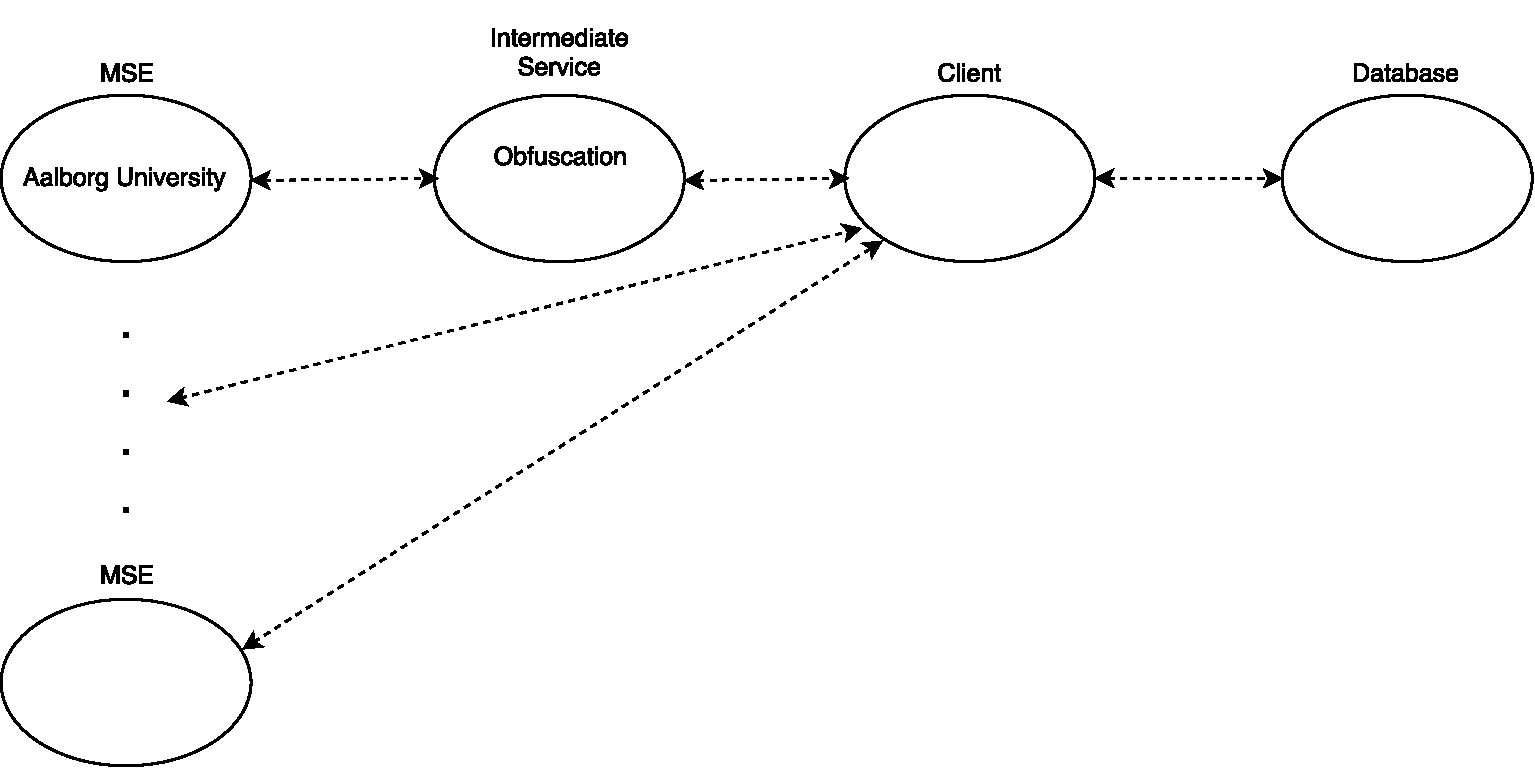
\includegraphics[scale=0.7]{graphics/ciscoNew.pdf}
		\caption{Cisco systems}
		\label{fig:cisco_systems}
	\end{center} 
\end{figure}
\Cref{fig:cisco_systems} shows how the information flow is intended. The client connecting to the Cisco services can function as a server that requests data from all Cisco services that we have access to. Alternatively, a server can be implemented for each Cisco service. However, this solution has several downsides. First, it means corporations supplying the multi-project with information will need to have a server running, which requires maintenance. Second, this solution is not scalable. The server running the aSTEP database will potentially be overloaded, as it has to handle each individual Cisco system sending information. As more Cisco systems are added, there will be less time to process received data. An alternative approach is to have the aSTEP database server request data using a round robin approach, however, with an increase in connected Cisco systems, the interval at which we receive new information from a given system also increases.

The optimal solution to this issue is to create a hierarchy of servers, such that the database server only receives data from a limited amount of intermediate servers, each of which also receive information from an amount of sources. During the start up of the aSTEP multi-project we have access to a single Cisco MSE system, and as such we will not focus on building this hierarchy. However, as the project grows and additional Cisco systems are integrated, it will eventually become a necessity.

\section{The Intermediate Server}\label{sec:future_intermediate}
As we are working on developing these tools to gather data, Cisco are further developing MSE. It is likely that new functionality has been added once development continues on this project, and it is therefore suggested that MSE is updated. The documentation for the newest version can always be found online, including the RESTful api documentation. From what we experienced, the documentation for the RESTful api is very poor, and requires additional effort to test functionality and acquire a good understanding of the api. Newer versions of MSE have some features that initially appear useful, but require a closer look to determine whether the project can make use it. We have chosen not to put effort into examining these features, as the documentation is very poor and easily misunderstood, and we have had very limited access to a system where we could test functionality.

One slightly obscure feature that MSE offers is to obfuscate MAC addresses. We do not know whether this is a binary setting, or if it is possible to configure this in more advanced ways. Similarly, MSE also offer the ability to subscribe to movement, such that subscribers are notified when movement occurs. However, this requires additional configuration on the MSE side, as well as a server that MSE can notify. Lastly, we suspect it might be possible to simply request positioning for the devices that have changed positions recently. We suggest these features are further explored.

\section{The Future of Our IPS}\label{sec:futureSystem}
As described in \cref{sec:ourSys} we have been working on building our own IPS. However, it was not possible for us to finish it as we encountered a significant difficulty. The obstacle we encountered was not being able to acquire the RSSI, and thus making it impossible for us to make further meaningful progress on our system within the remaining time limit. We do however believe it would be a fitting and interesting task for future developers.

The first step, if someone is to furtherer develop the system, should be to acquire the RSSI for devices connected to the network. The next step should be to expand the range of attainable devices by allowing multiple access points. From there is should be possible to calculate the distance between each access point based on the signal strength. This calculation can be performed by utilising one of the methods described in \cref{sec:tracking_approach}. By implementing these features it would be possible to calculate the positions of devices on the network, which we believe would be a crucial component of creating the system.

If the described features were implemented, a set of secondary functionality could be considered. The system could be expanded to receive the signal strength for all devices within the networks perimeter, connected or not. This would allow the system to track everyone within its coverage and thereby give it a more accurate view of the area.
Another beneficial feature the system could support, is be to calculate an estimate of how likely it is that the found locations are correct. This estimate could be similar to that the MSE provides with its \textit{confidenceFactor} described in \cref{sec:class_design}. This estimate will be useful for comparing the system's precision with other systems as descried in \cref{sec:ourSys}. 

\section{Coordinate Formats}
As described in \cref{sec:geo_coordinates}, there are three formats for geographical coordinates. We have chosen to provide the decimal degree format because it is the format used by the outdoor location groups and the format requested by the application group utilising indoor positioning.
However, future applications as well as future development on existing applications may need other formats. We have in \cref{sec:geo_coordinates} provided the necessary calculations to change the format. These calculations can be used in the future to implement the api.
\section{Security}\label{sec:fucture_secure}
More features could be implemented to further security in our system, as discussed in \cref{sec:secure}. We believe this is something for future students to focus on, and to implement as we handle sensitive information which should be handled in the best possible we.

\subsection{HTTPS on Intermediate Server}
We believe the most significant improvement future students can make to further security in this system would be to implement HTTPS on the intermediate server.
\section{Integration Test}\label{int_testing}
As of now the tests are made as unit tests, as described at \cref{subsec:unit_testing}, which is insufficient because of how the components of the system interacts.

An integration test is a set of unit tests that are aggregated to form a component \cite{msdn_it}. This type of tests would be beneficial for the system as all of the network communication methods are heavily intertwined within each other. This is apparent when analysing the data flow throughout the components that utilises these methods. It is possible to continue using the JUnit test suite for these tests.

One could argue that instead of relying on integration tests, it would be better to refactor the methods and components such that they are more atomic. By doing so, it would be easier to create likewise atomic unit tests that accompany the new refactored methods. This would not remove the need of integration tests as they are the next logical step in the software's life cycle as they are useful for testing major parts of the system. 


%Har vi husket at nævne de manglende unit tests i konklusionen?w

%%% CONCLUSION %%%
\chapter{Conclusion}
% Hvad har vi lavet?
In the course of this project we have build an ILBS which is capable of delivering indoor positioning data in real-time from Wi-Fi devices inside a set perimeter. This is done utilising a RESTFful service to communicate with a Cisco MSE service from which we are able to transfer and process the captured data. After the data is processed it is send to a database of which other aSTEP developers are responsible for. The data can then be requested by the different application and API developing groups.

% Sprint 1
In order to acquire mock data for aSTEP we chose to integrate MSE for the indoor positioning system as it was the most convenient choice. MSE was already installed at campus and the functionality it offers was sufficient to our needs. The data is processed and modified before it reaches the database as we had to obfuscate some of the sensitive personal data. This was done because of a demand from the MSE administrator and the Danish law of \textit{Directive on privacy and electronic communications}. As of such it was decided to obfuscate the sensitive person data of those users that did not consent.

% Sprint 2
The client was build to acquire data from multiple MSE services, as well as our intimidate server, and for sending data to the database. The client was designed to be robust and flexible, which was achieved by providing it with mechanisms for handling errors and by implementing a RESTful service for user inputs.

% Sprint 3
The foundation for a small tracking system was laid, with the future goal of being comparable with MSE in terms of the precision of the geographical coordinates. % Hvad er der mere at sige?
% Sprint 4 + resten
In order to give future students a smooth start, when they take ownership of the project, a set of precautions have been made. This involves code documentation, unit tests, the section \nameref{sec:catchup} and the various "How-to"s that have been made for this project's wiki at GitLab. 

Even tough we did not complete our own IPS, we will conclude that the project was a success. It was possible to deliver relevant positional data to the multi-project with the combined effort of the systems we made thus completing our primary goal. Valuable experience was gained by cooperating with the other members of the multi-project by doing numerous minor collaborations and other team oriented tasks.


%%%% Appendiks %%%%
\appendix														% Appendiks/bilag start - giver chapter bogstaver i stedet for tal
\phantomsection													% Kunstigt afsnit, som hyperlinks kan 'holde fast i'
%\pdfbookmark[0]{Appendiks}{appendiks}							% Tildeler en klikbar bookmark til den endelige PDF
\begin{lstlisting}[caption={TCP Data Package},label={lst:data_dump},mathescape]
***********************TCP Packet*************************
IP Header
|-IP Version        : 4
|-IP Header Length  : 5 DWORDS or 20 Bytes
|-Type Of Service   : 0
|-IP Total Length   : 140  Bytes(Size of Packet)
|-Identification    : 28418
|-TTL      : 128
|-Protocol : 6
|-Checksum : 33246
|-Source IP        : 172.26.120.216
|-Destination IP   : 172.26.120.126

TCP Header
|-Source Port      : 10523
|-Destination Port : 445
|-Sequence Number    : 1193890339
|-Acknowledge Number : 2211150917
|-Header Length      : 5 DWORDS or 20 BYTES
|-Urgent Flag          : 0
|-Acknowledgement Flag : 1
|-Push Flag            : 1
|-Reset Flag           : 0
|-Synchronise Flag     : 0
|-Finish Flag          : 0
|-Window         : 251
|-Checksum       : 22600
|-Urgent Pointer : 0

DATA Dump                         
IP Header
45 00 00 8C 6F 02 00 00 80 06 81 DE AC 1A 78 D8         E...o...\euro.....x.
AC 1A 78 7E                                             ..x~
TCP Header
29 1B 01 BD 47 29 52 23 83 CB 7C 45 50 18 00 FB         )...G)R#..|EP...
58 48 00 00                                             XH..
Data Payload
00 00 00 60 FE 53 4D 42 40 00 01 00 00 00 00 00         ...`.SMB@.......
0F 00 01 00 30 00 00 00 00 00 00 00 2E 00 00 00         ....0...........
00 00 00 00 FF FE 00 00 B5 F6 4C 26 43 44 3D 31         ..........L\&CD=1
00 00 00 00 00 00 00 00 00 00 00 00 00 00 00 00         ................
00 00 00 00 20 00 01 00 20 00 00 00 58 36 6D 8E         .... ... ...X6m.
00 00 00 00 E8 98 D8 7D 00 00 00 00 03 00 00 00         .......}........
00 00 00 00                                             ....
###########################################################
\end{lstlisting}

%%Glossary
\printglossary[style=long]

%% List of figures
\listoffigures

%% list of tables
\listoftables

%% List of listings
\lstlistoflistings

%% List of Fx notes
%\newpage
%\listoffixmes

%%%% Kilder %%%%
\begingroup
\raggedright
%    \bibliography{bib}							% Litteraturlisten inkluderes
\printbibliography
\endgroup

\end{document}	